\documentclass[a4paper, 10pt]{article}

\usepackage{amsmath}
\usepackage{amsfonts}
\usepackage{amssymb}
\usepackage{mathtools}
\usepackage{graphicx}
\usepackage{physics}

\begin{document}

\title{Sample Document}
\author{hari64boli64}
\date{\today}
\maketitle

\section{Rename Command}

\begin{equation}\label{eq:1}
    a = b
\end{equation}

\begin{equation*}
    c = d
\end{equation*}

\begin{align}
    e & = \begin{dcases}
              f & \text{if } g = h \\
              i & \text{if } j = k
          \end{dcases} \\
    l & = m \notag
\end{align}

\begin{figure*}[h] % comment
    \centering
    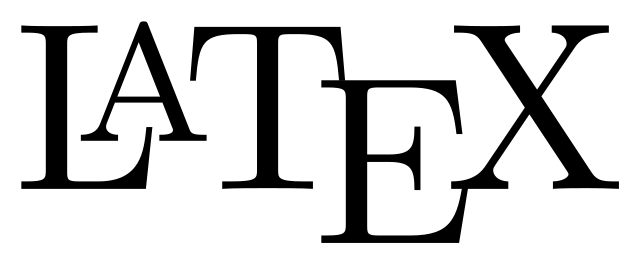
\includegraphics[width=0.5\columnwidth]{../images/sample.png}
    \caption{Sample Figure}
    \label{fig:1}
\end{figure*}

Sample figure is shown in Figure~\ref{fig:1}.

\section{Ask Wolfram Alpha}

Select a line. Then, press \texttt{Ctrl + Shift + P} and type \texttt{askWolframAlpha}.
\begin{gather*}
    \sum_{n=1}^{\infty} \frac{1}{n^2} \\
    \int_{-\infty}^{\infty} e^{-x^2} \dd x \\
    \left(1+\left(1+\left(1+x\right)^2\right)^2\right) \\
\end{gather*}

The Wolfram Alpha page with adjusted expressions will open as in Figure~\ref{fig:2}.
\begin{figure}[htbp]
    \centering
    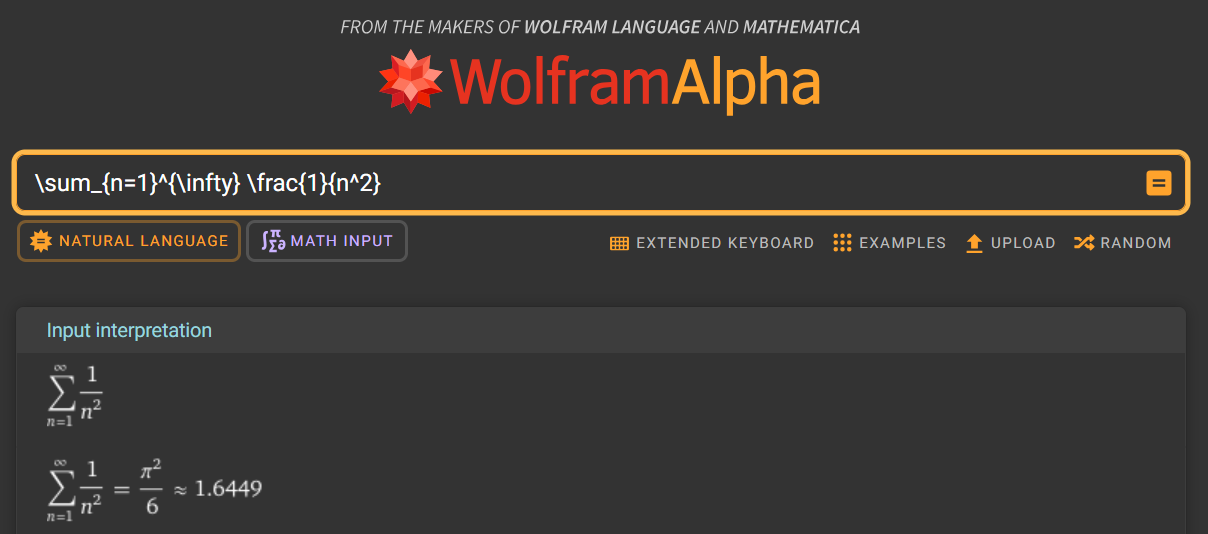
\includegraphics[width=\columnwidth]{../images/WolframAlpha.png}
    \caption{Wolfram Alpha}
    \label{fig:2}
\end{figure}

\end{document}
